\documentclass[11pt,a4paper]{article}
\usepackage{graphicx}
\usepackage{amsmath}
\usepackage{amssymb}
\usepackage{multicol}
\usepackage{tcolorbox}
\usepackage{xcolor}
\usepackage{geometry}
\usepackage{tikz}
\usepackage{array}
\usetikzlibrary{shapes.geometric, arrows}
\geometry{margin=0.8in}

% Define colors
\definecolor{mlblue}{RGB}{31, 119, 180}
\definecolor{mlorange}{RGB}{255, 127, 14}
\definecolor{mlgreen}{RGB}{44, 160, 44}
\definecolor{mlred}{RGB}{214, 39, 40}
\definecolor{mlpurple}{RGB}{148, 103, 189}
\definecolor{mlyellow}{RGB}{241, 196, 15}

\title{\Large\textbf{Discovery Learning 3: Innovation Safari}\\
\vspace{0.3em}
\normalsize From One Challenge to Many Ideas to Few Solutions}
\author{Machine Learning for Smarter Innovation - Pre-Lecture Activity}
\date{}

\begin{document}
\maketitle
\vspace{-1em}

\begin{tcolorbox}[colback=mlpurple!10, colframe=mlpurple!50, title=Learning Objectives]
\small
By completing this activity, you will discover:
\begin{itemize}
\item How innovation naturally expands then converges (the diamond pattern)
\item Why we need systematic filtering at scale
\item How clustering helps organize the innovation process
\end{itemize}
\end{tcolorbox}

\section*{The Innovation Diamond Journey}

\begin{center}
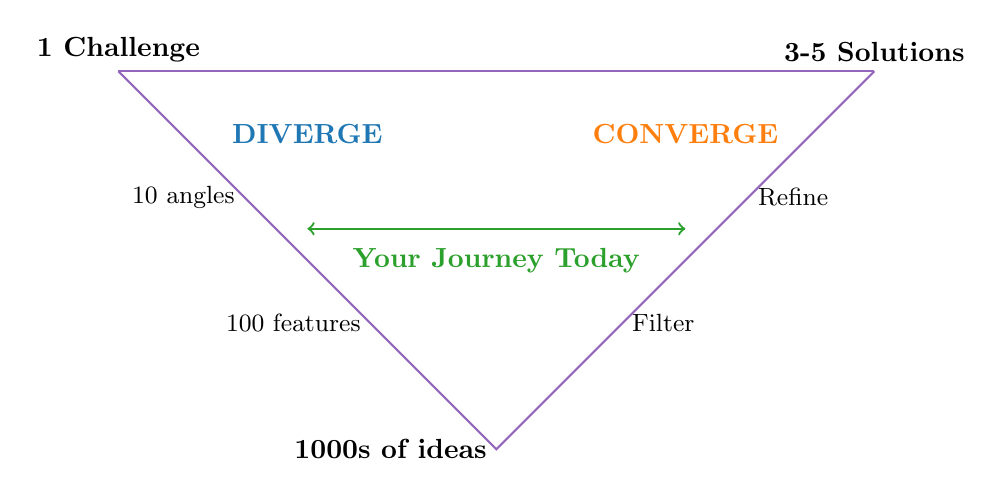
\begin{tikzpicture}[scale=0.8]
% Diamond shape
\draw[thick, mlpurple] (0,6) -- (2,4) -- (4,2) -- (6,0) -- (8,2) -- (10,4) -- (12,6);
\draw[thick, mlpurple] (0,6) -- (12,6);

% Labels
\node[above] at (0,6) {\textbf{1 Challenge}};
\node[left] at (2,4) {\small 10 angles};
\node[left] at (4,2) {\small 100 features};
\node[left] at (6,0) {\textbf{1000s of ideas}};
\node[right] at (8,2) {\small Filter};
\node[right] at (10,4) {\small Refine};
\node[above] at (12,6) {\textbf{3-5 Solutions}};

% Phase labels
\node[mlblue] at (3,5) {\textbf{DIVERGE}};
\node[mlorange] at (9,5) {\textbf{CONVERGE}};
\draw[<->, thick, mlgreen] (3,3.5) -- (9,3.5);
\node[mlgreen] at (6,3) {\textbf{Your Journey Today}};
\end{tikzpicture}
\end{center}

\section*{Phase 1: DIVERGE - Expansion of Ideas}

\subsection*{Your Challenge}
\begin{tcolorbox}[colback=mlpurple!20, colframe=mlpurple!70]
\Large\textbf{``Reduce plastic waste in universities''}
\end{tcolorbox}

\subsection*{Exercise 1: Rapid Ideation (5 minutes)}
Generate at least 20 different ideas to address this challenge. Don't judge - just create!

\newcommand{\Circle}{\tikz\draw[black, thick] (0,0) circle (.5ex);}

\begin{center}
\footnotesize
\begin{tabular}{|p{5.5cm}|c|c|c|c|c|}
\hline
\textbf{Idea} & \textbf{Cost} & \textbf{Scale} & \textbf{Tech} & \textbf{Time} & \textbf{Impact} \\
 & Low/Med/High & S/M/L & Y/N & Quick/Long & 1-5 \\
\hline
1. \underline{\hspace{5cm}} & \Circle & \Circle & \Circle & \Circle & \Circle \\
\hline
2. \underline{\hspace{5cm}} & \Circle & \Circle & \Circle & \Circle & \Circle \\
\hline
3. \underline{\hspace{5cm}} & \Circle & \Circle & \Circle & \Circle & \Circle \\
\hline
4. \underline{\hspace{5cm}} & \Circle & \Circle & \Circle & \Circle & \Circle \\
\hline
5. \underline{\hspace{5cm}} & \Circle & \Circle & \Circle & \Circle & \Circle \\
\hline
6. \underline{\hspace{5cm}} & \Circle & \Circle & \Circle & \Circle & \Circle \\
\hline
7. \underline{\hspace{5cm}} & \Circle & \Circle & \Circle & \Circle & \Circle \\
\hline
8. \underline{\hspace{5cm}} & \Circle & \Circle & \Circle & \Circle & \Circle \\
\hline
9. \underline{\hspace{5cm}} & \Circle & \Circle & \Circle & \Circle & \Circle \\
\hline
10. \underline{\hspace{5cm}} & \Circle & \Circle & \Circle & \Circle & \Circle \\
\hline
11. \underline{\hspace{5cm}} & \Circle & \Circle & \Circle & \Circle & \Circle \\
\hline
12. \underline{\hspace{5cm}} & \Circle & \Circle & \Circle & \Circle & \Circle \\
\hline
13. \underline{\hspace{5cm}} & \Circle & \Circle & \Circle & \Circle & \Circle \\
\hline
14. \underline{\hspace{5cm}} & \Circle & \Circle & \Circle & \Circle & \Circle \\
\hline
15. \underline{\hspace{5cm}} & \Circle & \Circle & \Circle & \Circle & \Circle \\
\hline
16. \underline{\hspace{5cm}} & \Circle & \Circle & \Circle & \Circle & \Circle \\
\hline
17. \underline{\hspace{5cm}} & \Circle & \Circle & \Circle & \Circle & \Circle \\
\hline
18. \underline{\hspace{5cm}} & \Circle & \Circle & \Circle & \Circle & \Circle \\
\hline
19. \underline{\hspace{5cm}} & \Circle & \Circle & \Circle & \Circle & \Circle \\
\hline
20. \underline{\hspace{5cm}} & \Circle & \Circle & \Circle & \Circle & \Circle \\
\hline
\end{tabular}
\end{center}

\subsection*{Exercise 2: Natural Grouping}
Look at your 20 ideas. Which ones naturally belong together? Create 3-5 groups below:

\begin{center}
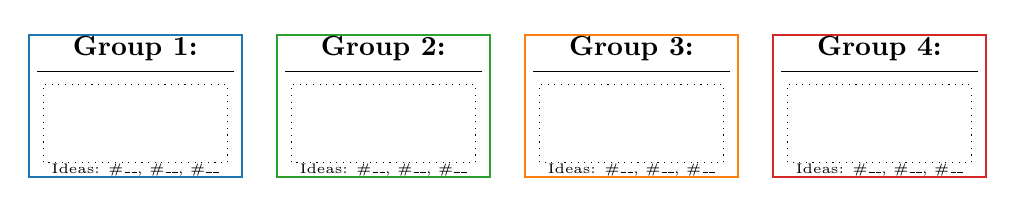
\begin{tikzpicture}[scale=0.9]
% Group boxes
\draw[thick, mlblue] (0,0) rectangle (3,2);
\node at (1.5,1.8) {\textbf{Group 1:}};
\node at (1.5,1.5) {\underline{\hspace{2.5cm}}};
\draw[dotted] (0.2,0.2) rectangle (2.8,1.3);
\node[font=\tiny] at (1.5,0.1) {Ideas: \#\_\_, \#\_\_, \#\_\_};

\draw[thick, mlgreen] (3.5,0) rectangle (6.5,2);
\node at (5,1.8) {\textbf{Group 2:}};
\node at (5,1.5) {\underline{\hspace{2.5cm}}};
\draw[dotted] (3.7,0.2) rectangle (6.3,1.3);
\node[font=\tiny] at (5,0.1) {Ideas: \#\_\_, \#\_\_, \#\_\_};

\draw[thick, mlorange] (7,0) rectangle (10,2);
\node at (8.5,1.8) {\textbf{Group 3:}};
\node at (8.5,1.5) {\underline{\hspace{2.5cm}}};
\draw[dotted] (7.2,0.2) rectangle (9.8,1.3);
\node[font=\tiny] at (8.5,0.1) {Ideas: \#\_\_, \#\_\_, \#\_\_};

\draw[thick, mlred] (10.5,0) rectangle (13.5,2);
\node at (12,1.8) {\textbf{Group 4:}};
\node at (12,1.5) {\underline{\hspace{2.5cm}}};
\draw[dotted] (10.7,0.2) rectangle (13.3,1.3);
\node[font=\tiny] at (12,0.1) {Ideas: \#\_\_, \#\_\_, \#\_\_};
\end{tikzpicture}
\end{center}

\newpage

\section*{Phase 2: CONVERGE - Filtering to Excellence}

\subsection*{Exercise 3: The Filtering Funnel}
Apply successive filters to narrow down to your best 3 ideas:

\begin{center}
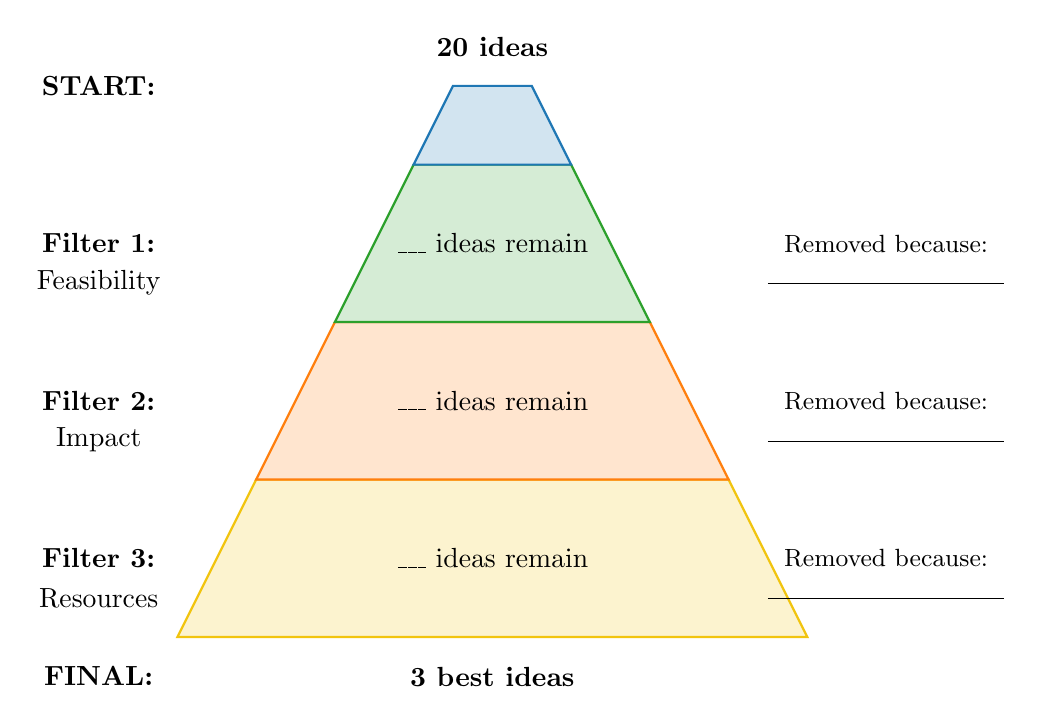
\begin{tikzpicture}[scale=1]
% Funnel shape
\draw[thick, mlyellow, fill=mlyellow!20] (2,0) -- (10,0) -- (9,2) -- (3,2) -- cycle;
\draw[thick, mlorange, fill=mlorange!20] (3,2) -- (9,2) -- (8,4) -- (4,4) -- cycle;
\draw[thick, mlgreen, fill=mlgreen!20] (4,4) -- (8,4) -- (7,6) -- (5,6) -- cycle;
\draw[thick, mlblue, fill=mlblue!20] (5,6) -- (7,6) -- (6.5,7) -- (5.5,7) -- cycle;

% Labels
\node at (1,7) {\textbf{START:}};
\node at (6,7.5) {\textbf{20 ideas}};

\node at (1,5) {\textbf{Filter 1:}};
\node at (1,4.5) {Feasibility};
\node at (6,5) {\_\_\_ ideas remain};
\node[font=\small] at (11,5) {Removed because:};
\node[font=\small] at (11,4.5) {\underline{\hspace{3cm}}};

\node at (1,3) {\textbf{Filter 2:}};
\node at (1,2.5) {Impact};
\node at (6,3) {\_\_\_ ideas remain};
\node[font=\small] at (11,3) {Removed because:};
\node[font=\small] at (11,2.5) {\underline{\hspace{3cm}}};

\node at (1,1) {\textbf{Filter 3:}};
\node at (1,0.5) {Resources};
\node at (6,1) {\_\_\_ ideas remain};
\node[font=\small] at (11,1) {Removed because:};
\node[font=\small] at (11,0.5) {\underline{\hspace{3cm}}};

\node at (1,-0.5) {\textbf{FINAL:}};
\node at (6,-0.5) {\textbf{3 best ideas}};
\end{tikzpicture}
\end{center}

\subsection*{Your Top 3 Solutions:}
\begin{enumerate}
\item \underline{\hspace{10cm}}
\item \underline{\hspace{10cm}}
\item \underline{\hspace{10cm}}
\end{enumerate}

\section*{Discovery Moment: Pattern Recognition}

\begin{tcolorbox}[colback=mlgreen!10, colframe=mlgreen!50, title=What Patterns Emerged?]
Looking at your groups and filtering process:
\begin{itemize}
\item Which group had the most survivors? \underline{\hspace{5cm}}
\item What feature best predicted success? \underline{\hspace{5cm}}
\item What surprised you about what got filtered? \underline{\hspace{4cm}}
\end{itemize}
\end{tcolorbox}

\section*{The Scale Problem}

\begin{center}
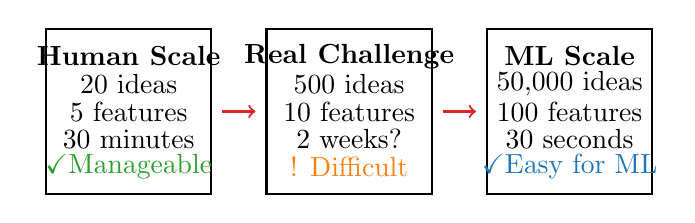
\begin{tikzpicture}[scale=0.7]
% Human scale
\draw[thick] (0,0) rectangle (3,3);
\node at (1.5,2.5) {\textbf{Human Scale}};
\node at (1.5,2) {20 ideas};
\node at (1.5,1.5) {5 features};
\node at (1.5,1) {30 minutes};
\node[mlgreen] at (1.5,0.5) {\checkmark Manageable};

% Challenge scale
\draw[thick] (4,0) rectangle (7,3);
\node at (5.5,2.5) {\textbf{Real Challenge}};
\node at (5.5,2) {500 ideas};
\node at (5.5,1.5) {10 features};
\node at (5.5,1) {2 weeks?};
\node[mlorange] at (5.5,0.5) {! Difficult};

% ML scale
\draw[thick] (8,0) rectangle (11,3);
\node at (9.5,2.5) {\textbf{ML Scale}};
\node at (9.5,2) {50,000 ideas};
\node at (9.5,1.5) {100 features};
\node at (9.5,1) {30 seconds};
\node[mlblue] at (9.5,0.5) {\checkmark Easy for ML};

% Arrows
\draw[->, thick, mlred] (3.2,1.5) -- (3.8,1.5);
\draw[->, thick, mlred] (7.2,1.5) -- (7.8,1.5);
\end{tikzpicture}
\end{center}

\section*{Reflection Questions}

\begin{enumerate}
\item \textbf{Grouping Challenge:} Did all your ideas fit neatly into groups? What about the ``weird'' ones?\\
\vspace{0.3em}
\underline{\hspace{14cm}}\\
\underline{\hspace{14cm}}

\item \textbf{Filter Fairness:} Did good ideas get eliminated? How could better features prevent this?\\
\vspace{0.3em}
\underline{\hspace{14cm}}\\
\underline{\hspace{14cm}}

\item \textbf{Imagine Scale:} Your university collected 5,000 ideas from students. How would you even begin to organize them?\\
\vspace{0.3em}
\underline{\hspace{14cm}}\\
\underline{\hspace{14cm}}

\item \textbf{Pattern Prediction:} If a computer analyzed your 20 ideas, what patterns do you think it would find that you missed?\\
\vspace{0.3em}
\underline{\hspace{14cm}}\\
\underline{\hspace{14cm}}
\end{enumerate}

\begin{tcolorbox}[colback=mlpurple!10, colframe=mlpurple!50, title=Prepare for Next Class: The Innovation Diamond]
You've just experienced the innovation diamond:
\begin{itemize}
\item Started with 1 challenge
\item Expanded to 20+ ideas (imagine 5,000!)
\item Converged to 3 solutions
\end{itemize}

In our next lecture, you'll learn how machine learning can:
\begin{itemize}
\item Handle millions of ideas
\item Find patterns humans can't see
\item Optimize the filtering process
\item Ensure no good idea gets lost
\end{itemize}

\textbf{Think about:} What if we could analyze every innovation idea ever proposed at every university worldwide?
\end{tcolorbox}

\end{document}